\documentclass[aspectratio=169]{slide-ja}

\usepackage{physics}
\usepackage{caption}
\usepackage{subcaption}

\usepackage{algorithm}
\usepackage{algpseudocodex}
\usepackage{amsmath}
\usepackage{array}
\usepackage{bbm}
\usepackage{booktabs}
\usepackage{csvsimple} % csvreader

\graphicspath{{src/}}
\addbibresource{src/myref.bib}

\newcommand{\ispace}{\mathbb{D}^{m}}
\newcommand{\Prec}{\operatorname{acc}}
\newcommand{\Cov}{\operatorname{cov}}
\newcommand{\cands}{\bar{\mathcal{A}}}
\algnewcommand{\IIf}[1]{\State\algorithmicif\ #1\ \algorithmicthen\ }
\renewcommand{\algorithmicrequire}{\textbf{Input:}}
\renewcommand{\algorithmicensure}{\textbf{Output:}}


\newcommand{\dtrain}{D_{\mathrm{train}}}
\newcommand{\dtest}{D_{\mathrm{test}}}
\newcommand{\dmis}{D_{\mathrm{mis}}}
\newcommand{\dchange}{D_{\mathrm{change}}}

\title{雑誌会}
\author{大原玄嗣}
\institute{情報認識学研究室 M1}

\begin{document}

\begin{frame}
  \frametitle{発表の概要}
  \setbeamertemplate{section in toc}[ball unnumbered]
  \setcounter{tocdepth}{1} % show only chapters and sections in toc
  \tableofcontents
\end{frame}

\section[卒業研究 \\ R-LIME:\@~LIME法の矩形制約と最適化]{%
  卒業研究 「R-LIME:~LIME法の矩形制約と最適化」
 }

\subsection{研究の背景}
\begin{frame}
  \frametitle{研究の背景}
  \colorrect{red}{解釈可能な機械学習 (Interpretable Machine Learning)}
  \bigskip
  \begin{columns}[]
    \begin{column}{0.5\textwidth}
      \begin{itemize}
        \item 複雑な機械学習モデル (Black Box)
              \begin{itemize}
                \item 深層ニューラルネットワーク
                \item アンサンブルモデル
              \end{itemize}
              \smallskip
              \textrightarrow{}出力の根拠が\underline{解釈困難}
      \end{itemize}
      \centering
      \COLabel{complex}{}
    \end{column}
    \begin{column}{0.5\textwidth}
      \begin{itemize}
        \item 単純な機械学習モデル (White Box)
              \begin{itemize}
                \item 線形モデル
                \item 決定木
              \end{itemize}
              \smallskip
              \textrightarrow{}出力の根拠が\underline{解釈可能}
      \end{itemize}
      \centering
      \COLabel{simple}{}
    \end{column}
  \end{columns}
  \begin{tikzpicture}[remember picture,overlay]
    \draw (simple) edge [->, thick, bend left=20] node [midway, below]
      {\colorrect{blue}{局所近似によって解釈}} (complex);
  \end{tikzpicture}
\end{frame}

\subsection{関連研究}

\begin{frame}
  \frametitle{関連研究}
  \begin{itemize}
    \item LIME\footfullcite{ribeiro2016why}
    \item Anchor\footfullcite{ribeiro2018anchors}
    \item BELLA\footfullcite{radulovic2023bella}
          (Appendix: Page~\ref{frame:bella1},~\ref{frame:bella2})
  \end{itemize}
\end{frame}

\begin{frame}
  \frametitle{%
    関連研究1 — LIME
    \small{(Local Interpretable Model-agnostic Explanations)}
    \footfullcite{ribeiro2016why}
  }
  \begin{columns}[]
    \begin{column}{0.5\textwidth}
      \begin{enumerate}
        \item 着目点の周辺で摂動サンプルを生成
        \item 得られたサンプル集合で\\線形モデルを学習
      \end{enumerate}
    \end{column}
    \begin{column}{0.5\textwidth}
      \begin{figure}
        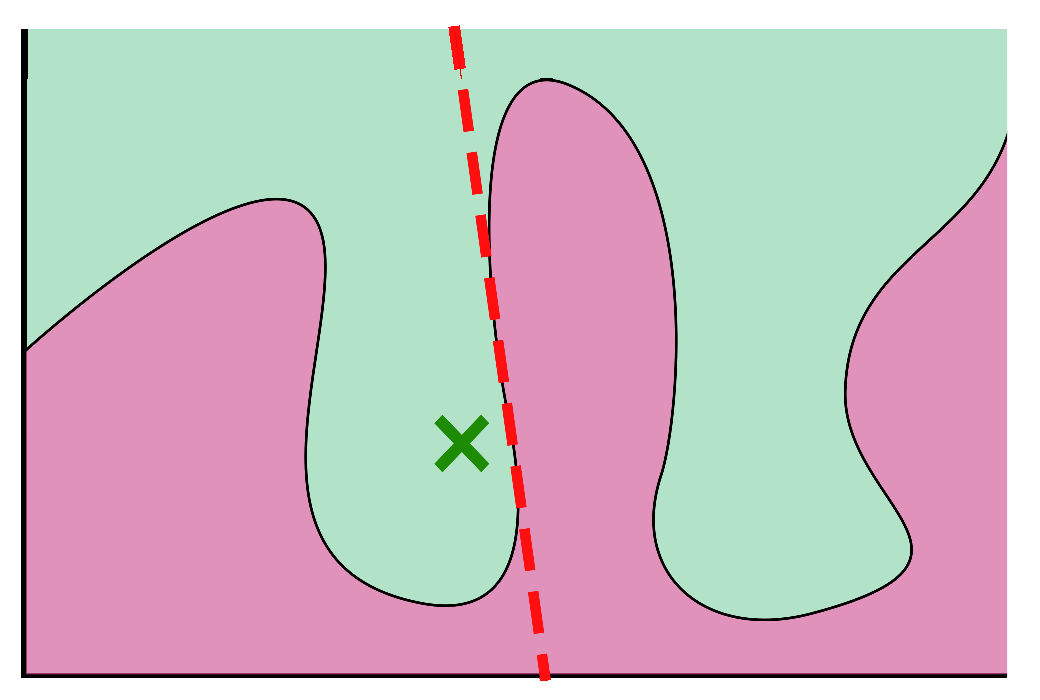
\includegraphics[scale=0.35]{visual-lime}
      \end{figure}
    \end{column}
  \end{columns}
\end{frame}

\begin{frame}
  \frametitle{関連研究1 — LIMEの出力例}
  \begin{columns}[]
    \begin{column}{0.35\textwidth}
      \vspace{4.2em}
      \begin{figure}
        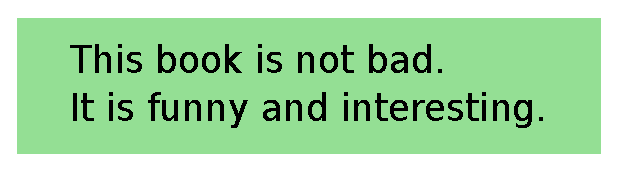
\includegraphics[width=\textwidth]{example-instance}
        \vspace{0.8em}
        \caption{%
          着目点の例.感情予測モデルはこの文章を``Positive''な文章と予測した.
        }
      \end{figure}
    \end{column}
    \begin{column}{0.4\textwidth}
      \begin{figure}
        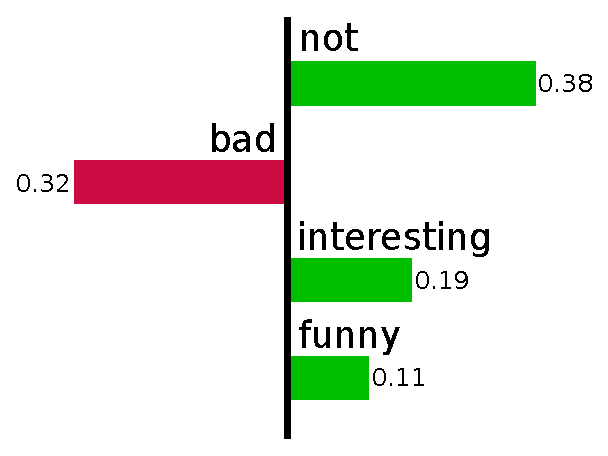
\includegraphics[width=0.9\textwidth]{example-lime}
        \caption{%
          着目点に対する感情予測モデルの予測に関して,LIMEが出力する説明の例.
        }
      \end{figure}
    \end{column}
  \end{columns}
\end{frame}

\begin{frame}
  \frametitle{関連研究1 — LIMEの問題点}
  \begin{columns}[]
    \begin{column}{0.4\textwidth}
      \underline{説明の適用範囲が示されない}

      \bigskip
      \begin{itemize}
        \item 説明から得られた知見は\\どの程度一般的なのか?
      \end{itemize}
    \end{column}
    \begin{column}{0.45\textwidth}
      \begin{figure}
        \includegraphics[width=\textwidth]{src/lime_drawback}
      \end{figure}
    \end{column}
  \end{columns}
\end{frame}

\begin{frame}
  \frametitle{関連研究2 — Anchor\footfullcite{ribeiro2018anchors}}
  \begin{columns}[]
    \begin{column}{0.5\textwidth}
      \begin{itemize}
        \item モデルの出力が高い確率で\\一致する矩形領域を探索
        \item 矩形領域を特徴量に関する\\述語の連言として表現\\
              \textit{\footnotesize{ex. Gender = ‘Male’ AND 20 <= Age < 30}}
      \end{itemize}

      \bigskip
    \end{column}
    \begin{column}{0.5\textwidth}
      \begin{figure}
        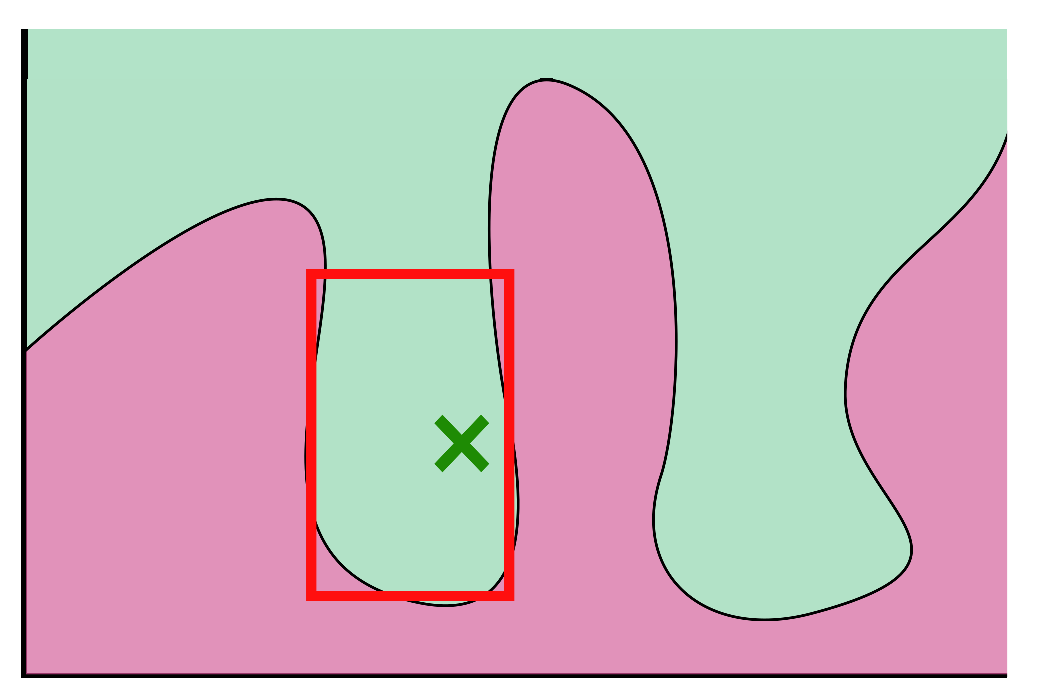
\includegraphics[scale=0.35]{visual-anchor}
      \end{figure}
    \end{column}
  \end{columns}
\end{frame}

\begin{frame}
  \frametitle{関連研究2 — Anchorの出力例}
  \begin{columns}[]
    \begin{column}{0.35\textwidth}
      \begin{figure}
        \centering
        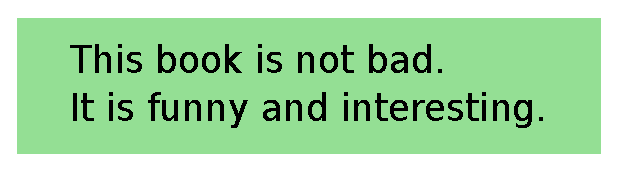
\includegraphics[width=\textwidth]{example-instance}
        \caption{%
          着目点の例.感情予測モデルはこの文章を``Positive''な文章と予測した.
        }
      \end{figure}
    \end{column}
    \begin{column}{0.4\textwidth}
      \vspace{0.7em}
      \begin{figure}
        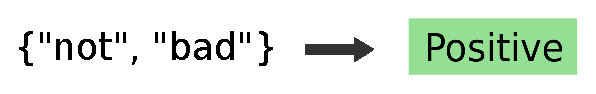
\includegraphics[width=\textwidth]{example-anchor}
        \vspace{-0.5em}
        \caption{%
          着目点に対する感情予測モデルの予測に関して,
          Anchor が出力する説明の例.
        }
      \end{figure}
    \end{column}
  \end{columns}
\end{frame}

\begin{frame}
  \frametitle{関連研究2 — Anchorの問題点}
  \begin{columns}[]
    \begin{column}{0.4\textwidth}
      \underline{説明から得られる知見が少ない}

      \bigskip
      \begin{itemize}
        \item 各特徴量の影響の大きさが \\ 示されない
      \end{itemize}
    \end{column}
    \begin{column}{0.5\textwidth}
      \begin{figure}
        \begin{subfigure}[t]{\textwidth}
          \centering
          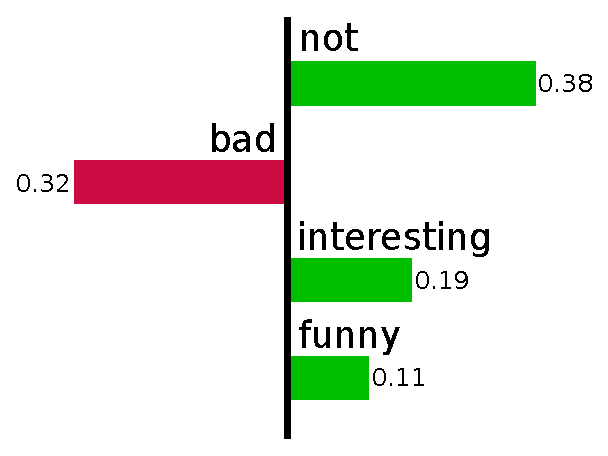
\includegraphics[scale=0.4]{example-lime}
        \end{subfigure}
        \begin{subfigure}[t]{\textwidth}
          \centering
          \vspace{0.5em}
          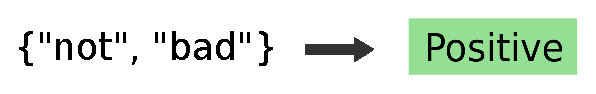
\includegraphics[scale=0.4]{example-anchor}
        \end{subfigure}
        \vspace{0.5em}
        \caption{感情予測モデルに対するLIMEとAnchorの出力の比較}
      \end{figure}
    \end{column}
  \end{columns}
\end{frame}

\begin{frame}
  \frametitle{研究の目的}
  \renewcommand{\arraystretch}{1.5}
  \tabcolsep=1.5em
  \begin{center}
    \begin{tabular}{cccc}
                & LIME         & Anchor       & 提案手法         \\
      \midrule
      特徴量重要度の提示 & \checkmark{} & \times{}     & \checkmark{} \\
      近似領域の最適化  & \times{}     & \checkmark{} & \checkmark{} \\
      近似領域の解釈性  & \times{}     & \checkmark{} & \checkmark{} \\
    \end{tabular}
  \end{center}

  \bigskip
  \underline{説明の解釈性}と\underline{説明の適用範囲の解釈性}を両立

  \smallskip
  \textrightarrow~\colorrect{red}{ユーザは説明から得られた知見を正当な範囲で活用できる}
\end{frame}

\begin{frame}
  \frametitle{提案手法: R-LIME (Ruled LIME)}
  \begin{columns}[]
    \begin{column}{0.45\textwidth}
      \colorrect{red}{\textbf{R-LIME} = LIME + Anchor}

      \bigskip
      \begin{itemize}
        \item 近似領域を矩形に
        \item 近似領域を特徴量に関する\\述語の連言として表現\\
              \textit{\footnotesize{ex. Gender = ‘Male’ AND 20 <= Age < 30}}
      \end{itemize}
    \end{column}
    \begin{column}{0.55\textwidth}
      \begin{figure}
        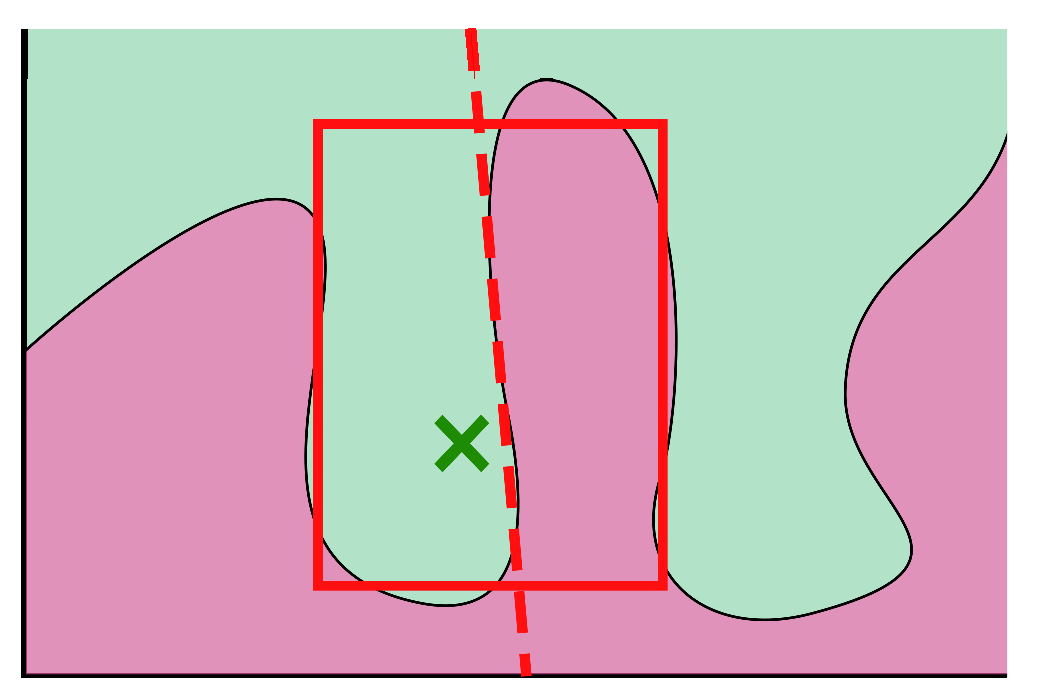
\includegraphics[scale=0.35]{visual-rlime3}
      \end{figure}
    \end{column}
  \end{columns}
\end{frame}

\begin{frame}
  \frametitle{提案手法: 問題設定}
  \vspace{-1.4em}
  \begin{align*}
     & \text{$m$次元入力空間 (離散化済み)} &  & \ispace             \\
     & \text{ブラックボックス分類器}       &  & f:\ispace\to\{0,1\} \\
     & \text{着目点}               &  & x\in\ispace         \\
     & \text{入力空間上の分布}          &  & \mathcal{D}         \\
     & \text{可能な線形近似モデルの全体}     &  & G
  \end{align*}

  ルール … 特徴量に関する述語の連言
  \vspace{-0.5em}
  \begin{equation*}
    A(z)=a_{i_1}(z)\wedge a_{i_2}(z)\wedge\dots\wedge a_{i_k}(z),\quad
    a_i(z)=\mathbbm{1}_{z_i=x_i}
  \end{equation*}
\end{frame}

{%
\vfuzz=13.08765pt
\begin{frame}
  \frametitle{提案手法: 問題設定}
  \bigskip
  \bigskip
  \bigskip

  \begin{alignat*}{2}
     & \text{ルール$A$の精度}  & \quad & \Prec(A)=\underset{g\in G}{\max}
    \ \mathbb{E}_{z\sim\mathcal{D}(z|A)}[\mathbbm{1}_{f(z)=g(z)}]
    \COLabel{prec}{}
    \\
     & \text{ルール$A$の被覆度} & \quad & \operatorname{cov}(A)=
    \mathbb{E}_{z\sim\mathcal{D}(z)}[A(z)]
    \COLabel{cov}{}
    \\
    \\
     & \text{最適化問題}      & \quad & \colorrect{red}{$
        \tilde{A}=\underset{A\ s.t.
          \ P(\Prec(A)\ge\tau)\ge1-\delta,A(x)=1}  % chktex 36
        {\arg\max}\operatorname{cov}(A)  % chktex 36
      $}
    \COLabel{problem}{}
    \\
  \end{alignat*}

  \begin{center}
    \underline{精度の下限制約の下で被覆度を最大化}
  \end{center}
  \CO{prec}{++ (1.0,1.2)}{矩形領域で学習された \\ 近似モデルの精度の期待値}
  \CO{cov}{++ (3.0,0.0)}{摂動サンプルが矩形領域に \\ 含まれる確率の期待値}
\end{frame}
}

\begin{frame}
  \frametitle{提案手法: アルゴリズム (ビームサーチ)}

  \bigskip
  \bigskip
  以下の処理を反復
  \begin{enumerate}
    \item $\mathcal{A}_i\gets$候補ルールの集合\COLabel{Cands}{}
    \item $\mathcal{A}_i\gets$精度が最大の$B$個のルール
          \COLabel{B-Cands}{}
    \item 精度制約を満たす被覆度最大のルールを選択 → 見つかれば終了
  \end{enumerate}
  \CO{Cands}{++ (2.5,1.2)}{%
    $\mathcal{A}_{i-1}$の中の各ルールに \\
    まだ含まれていない述語を1個加える
  }
  \CO{B-Cands}{++ (2.5,0.5)}{多腕バンディット問題の\\最適腕識別として解く}
  \vspace{-1em}
  \begin{figure}[t]
    \centering
    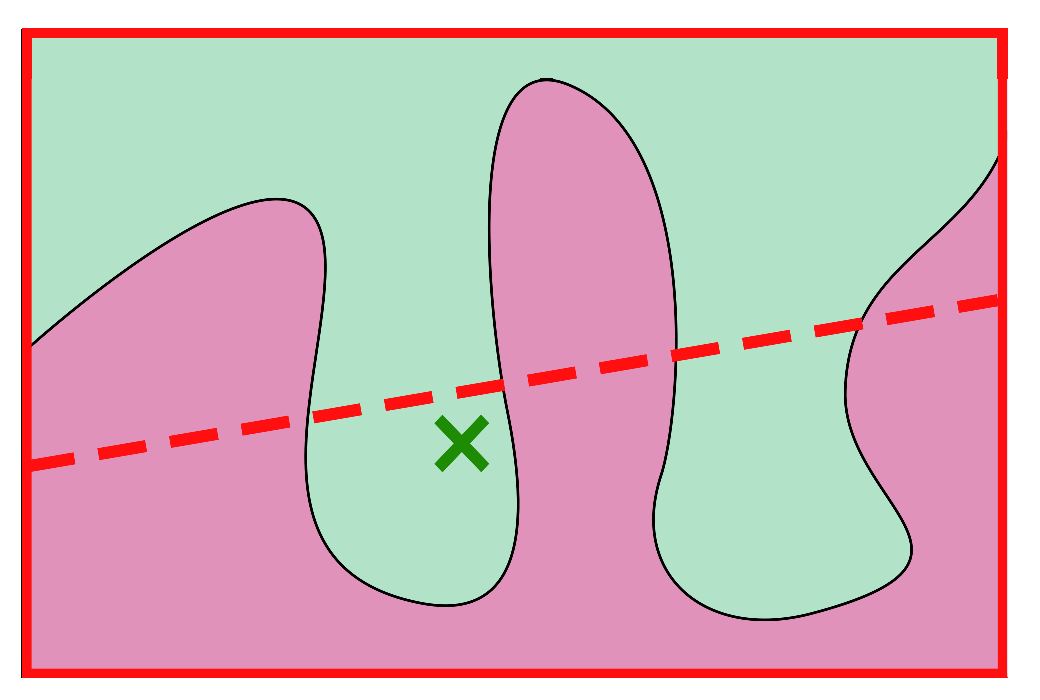
\includegraphics[width=0.31\textwidth]{visual-rlime1}
    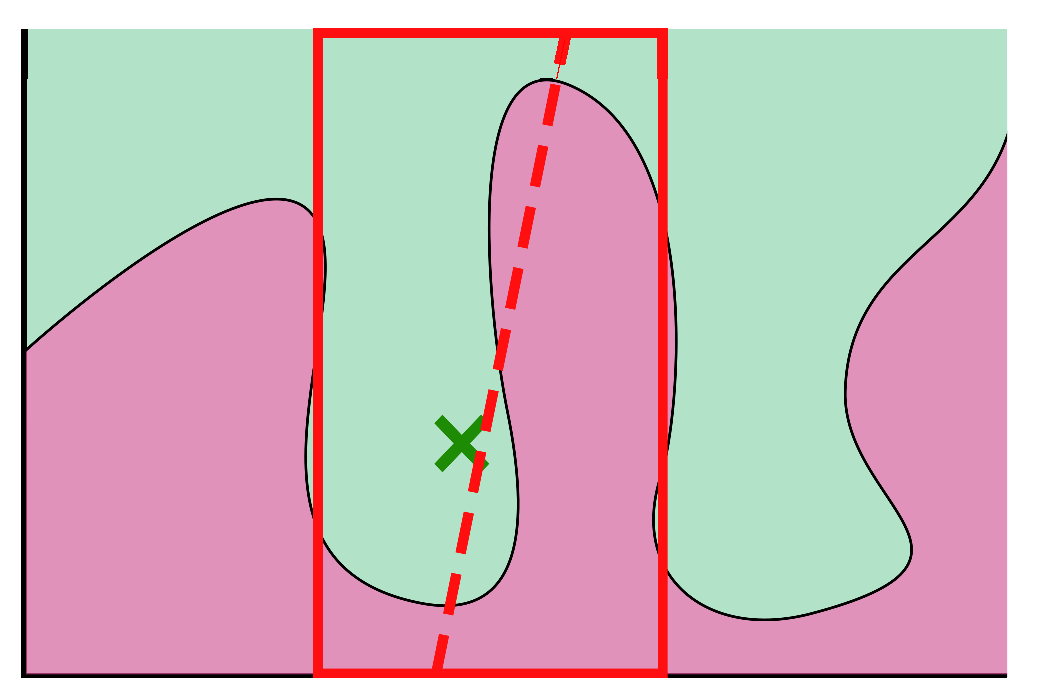
\includegraphics[width=0.31\textwidth]{visual-rlime2}
    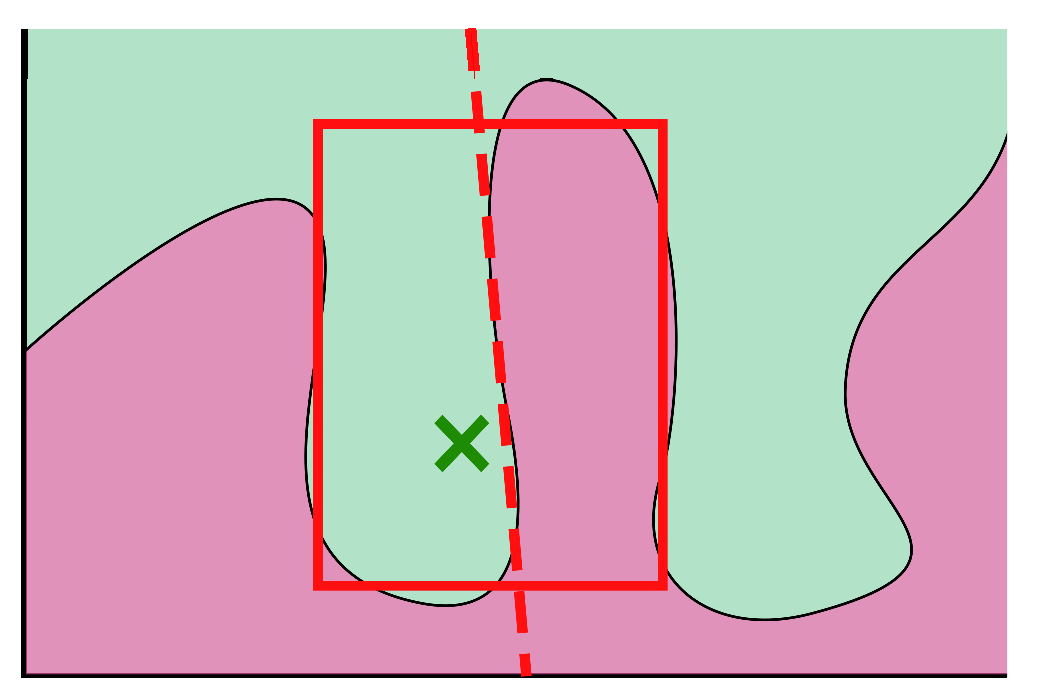
\includegraphics[width=0.31\textwidth]{visual-rlime3}
  \end{figure}
\end{frame}


\begin{frame}
  \frametitle{実験1~-~設定}
  実データセットについて,LIMEとR-LIMEを視覚的に比較
  \begin{itemize}
    \item recidivism データセット\footfullcite{schmidt1988predicting}を使用
    \item ブラックボックス分類器 (ランダムフォレスト) を学習
    \item データセットから抽出したインスタンスに対するLIMEとR-LIMEの説明を比較
  \end{itemize}
\end{frame}

\def\index{0012}
\def\dir{src/rlime-examples/examples}

\begin{frame}
  \frametitle{実験1~-~設定: 着目点となる入力}
  \renewcommand{\arraystretch}{0.80}
  \centering
  \footnotesize
  \begin{table}
    \begin{tabular}{p{14em}m{16em}}
      \toprule
      \csvreader[no head, late after line= \\]{%
        \dir/\index.csv
      }{}{\ifnum\thecsvrow=16\midrule\fi\csvcoli{} & \csvcolii}
      \bottomrule
    \end{tabular}
  \end{table}
\end{frame}

{%
\def\scale{0.42}

\begin{frame}
  \frametitle{実験1~-~結果: LIMEによる説明}
  ランダムフォレストの出力に対する各特徴量の寄与度を提示
  \bigskip
  \begin{figure}[b]
    \hspace{-5em}
    \includegraphics[scale=\scale]{\dir/lime-\index}
  \end{figure}
\end{frame}

\begin{frame}
  \frametitle{実験1~-~結果: 提案手法による説明 (閾値$\tau=0.70$)}
  既婚の受刑者のみに適用可能
  \begin{figure}
    \hspace{-5em}
    \includegraphics[scale=\scale]{\dir/newlime-\index-70}
  \end{figure}
\end{frame}

\begin{frame}
  \frametitle{実験1~-~結果: 提案手法による説明 (閾値$\tau=0.80$)}
  収監期間による制約が追加され,
  被覆度 (Coverage) は$\tau=0.70$のときに比べて減少
  \begin{figure}
    \hspace{-4.8em}
    \includegraphics[scale=\scale]{\dir/newlime-\index-80}
  \end{figure}
\end{frame}

\begin{frame}
  \frametitle{実験1~-~結果: 提案手法による説明 (閾値$\tau=0.90$)}
  被覆度が小さい → \underline{有用性は限定的}
  \begin{figure}
    \hspace{-2.3em}
    \includegraphics[scale=\scale]{\dir/newlime-\index-90}
  \end{figure}
\end{frame}
}

\begin{frame}
  \frametitle{実験2~-~設定}
  LIMEとR-LIMEの局所的な近似精度を比較
  \begin{itemize}
    \item recidivism データセットでランダムフォレストを学習
    \item データセットから無作為に抽出された100個のインスタンスに対して以下の処理を繰り返す
          \begin{itemize}
            \item LIMEとR-LIMEの説明を生成
            \item R-LIMEによって得られた矩形領域から10000個サンプリング
            \item 両者の近似精度を計算
          \end{itemize}
    \item 得られた近似精度の分布を比較
  \end{itemize}

\end{frame}

\begin{frame}
  \frametitle{実験2~-~結果}
  \begin{figure}
    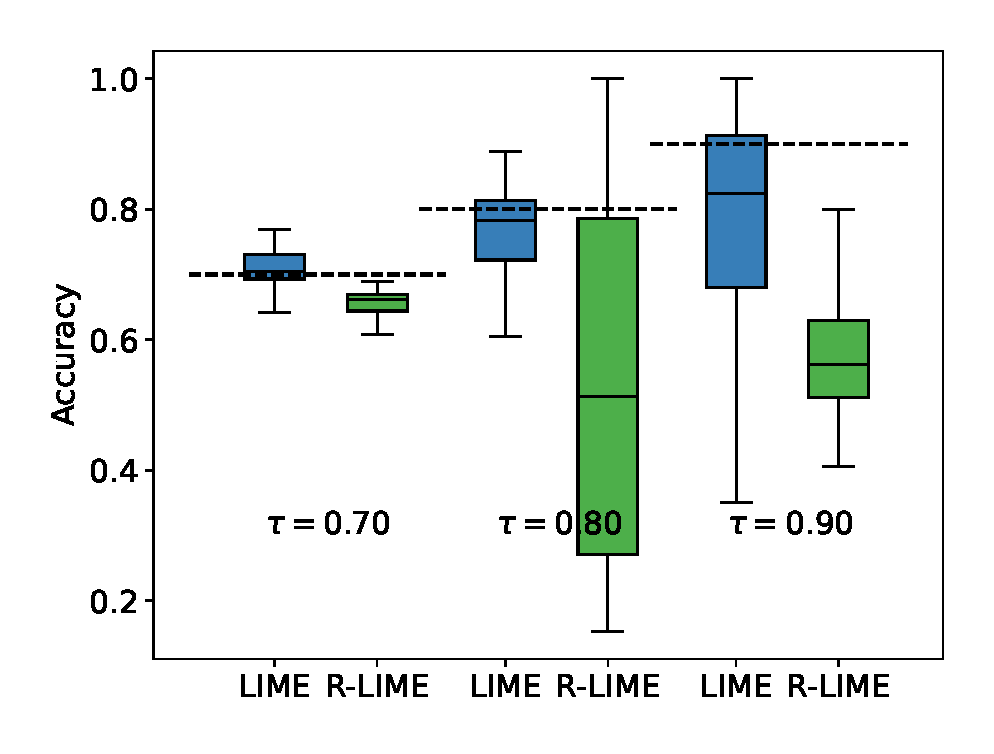
\includegraphics[height=142pt]{box_plot}
  \end{figure}
  R-LIMEは近似領域に適応した高精度の線形近似モデルを学習

  領域の取り方によっては,LIMEの説明は近似モデルとしてほとんど機能しない
\end{frame}

\begin{frame}
  \frametitle{結論}
  \renewcommand{\arraystretch}{1.5}
  \tabcolsep=1.5em
  \begin{center}
    \begin{tabular}{cccc}
                & LIME         & Anchor       & \textbf{R-LIME} \\
      \midrule
      特徴量重要度の提示 & \checkmark{} & \times{}     & \checkmark{}    \\
      近似領域の最適化  & \times{}     & \checkmark{} & \checkmark{}    \\
      近似領域の解釈性  & \times{}     & \checkmark{} & \checkmark{}    \\
    \end{tabular}
  \end{center}
  \center{%
    \colorrect{green}{%
      提案手法によって,ユーザは説明の適用範囲や \\
      信頼性・一般性を評価し正しく活用することができる
    }
  }
\end{frame}

\renewcommand\appendixname{Appendix}
\appendix
\section{Appendix}

\begin{frame}
  \frametitle{関連研究1 — LIMEのサンプリング}
  \begin{columns}[]
    \begin{column}{0.5\textwidth}
      \begin{enumerate}
        \item 着目点$x\in\mathbb{R}^d$を解釈可能な表現
              $x'\in{\{0,1\}}^{d'}$に変換
        \item $x'$の周辺で摂動$z_i'\in{\{0,1\}}^{d'}$を生成
        \item $z_i'$から$z_i\in\mathbb{R}^d$を復元
      \end{enumerate}
      \begin{flalign*}
        \pi_x(z_i)=\exp\left(\frac{-{d(x,z_i)}^2}{\delta^2}\right)
         & : z_i\text{~の重み}
      \end{flalign*}
    \end{column}
    \begin{column}{0.5\textwidth}
      \begin{figure}
        \includegraphics[width=\textwidth]{src/lime_sampling}
      \end{figure}
    \end{column}
  \end{columns}
\end{frame}

\begin{frame}
  \frametitle{%
    関連研究3 — BELLA
    \small{(Black box model Explanations by Local Linear Approximations)}
    \footfullcite{radulovic2023bella}
  }\label{frame:bella1}
  \begin{columns}[]
    \begin{column}{0.5\textwidth}
      \begin{enumerate}
        \item データセットに含まれる全てのデータと
              対象のインスタンスの距離を計算
        \item データセットの「最適な部分集合」を探索
        \item 得られた集合で,線形モデルを学習
      \end{enumerate}
    \end{column}
    \begin{column}{0.5\textwidth}
      \begin{figure}
        % \includegraphics[height=120pt]{bella}
      \end{figure}
    \end{column}
  \end{columns}
\end{frame}

\begin{frame}
  \frametitle{関連研究3 — BELLAの問題点}\label{frame:bella2}
  \underline{ブラックボックスモデルの学習に用いたデータセットを使う}
  \begin{itemize}
    \item プライバシーの制約に弱い
    \item 「どう学習したか」ではなく「どう振る舞うか」が知りたい
  \end{itemize}
  \underline{近似領域が解釈困難}
  \begin{itemize}
    \item データセットの部分集合からは,説明の適用範囲を判断できない
  \end{itemize}
\end{frame}

\begin{frame}
  \frametitle{関連研究と提案手法の比較}
  \renewcommand{\arraystretch}{1.5}
  \tabcolsep=1.5em
  \begin{center}
    \begin{tabular}{ccccc}
                & LIME         & Anchor       & BELLA        & \textbf{R-LIME} \\
      \midrule
      近似領域の最適化  & \times{}     & \checkmark{} & \checkmark{} & \checkmark{}    \\
      近似領域の解釈性  & \times{}     & \checkmark{} & \times{}     & \checkmark{}    \\
      特徴量重要度の提示 & \checkmark{} & \times{}     & \checkmark{} & \checkmark{}    \\
      摂動サンプルの生成 & \checkmark{} & \checkmark{} & \times{}     & \checkmark{}    \\
    \end{tabular}
  \end{center}
\end{frame}

\begin{frame}
  \begin{algorithm}[H]
    \caption{R-LIME}\label{alg:greedy-search}
\begin{algorithmic}[1]
	\Require{%
		Black-box model $f$, Target instance $x$,
		Distribution $\mathcal{D}$,
		Threshold $\tau$, Beam width $B$, Tolerance $\epsilon$,
		Confidence level $1-\delta$
	}
	\Ensure{%
		Rule $A^*$ satisfying Eq.~\eqref{eq:main-problem}
	}
	\State{$A^*\gets\textbf{null},\ \mathcal{A}_0\gets\emptyset,\ t\gets0$}
	% \Comment{%
	%   Initialize the set of candidate rules $\mathcal{A}_0$ to $\emptyset$
	% }
	\Comment{Initialize the set of candidate rules $\mathcal{A}_0$ to $\emptyset$}
	\While{$A^*=\textbf{null}$}
	\State$t\gets t+1$
	\State$\cands_t\gets$ \Call{GenerateCands}
	{$\mathcal{A}_{t-1}$}
	\State$\mathcal{A}_t\gets$ \Call{B-BestCands}
	{$\cands_{t},\mathcal{D},B,\epsilon,\delta$}
	\State$A^*\gets$ \Call{LargestCand}
	{$\mathcal{A}_t,\tau,\delta$}
	\EndWhile%
\end{algorithmic}

  \end{algorithm}
  \vspace{-2em}
  \begin{equation}
    \tilde{A}=\underset{A\ s.t.
      \ P(\Prec(A)\ge\tau)\ge1-\delta,A(x)=1}
    {\arg\max}\operatorname{cov}(A)
  \end{equation}
\end{frame}

\begin{frame}
  \begin{algorithm}[H]
    \caption{Generating new candidate rules}\label{alg:generate-cands}
\begin{algorithmic}[1]
	\Function{GenerateCands}{$\mathcal{A},x$}
	\IIf{$\mathcal{A}=\emptyset$}{\Return{$\{\mathit{true}\}$}}
	\Comment{An initial empty rule always returns $\mathit{true}$}
	\State$\cands\gets\emptyset$
	\ForAll{$A\in\mathcal{A}$}
	\ForAll{$a\in (T(x)\setminus A)$}
	\State$\cands\gets\bar{\mathcal{A}}\cup(A\wedge a)$
	\Comment{Get a new rule by adding a new predicate $a$ to $A$}
	\EndFor%
	\EndFor%
	\State\Return{$\cands$}
	\EndFunction%
\end{algorithmic}

  \end{algorithm}
\end{frame}

\begin{frame}
  \begin{algorithm}[H]
    \small
    \caption{%
	Searching rules with highest accuracy (KL-LUCB~\cite{kaufmann2013information})
}\label{alg:best-cands}
\begin{algorithmic}[1]
	\Function{B-BestCands}{$\cands,\mathcal{D},B,\epsilon,\delta$}
	\State\textbf{initialize} $\Prec,\Prec_{u},\Prec_{l}$ for $\forall A\in\cands$
	\State$\mathcal{A}\gets\Call{B-ProvisionallyBestCands}{\cands}$
	\Comment{$B$ rules with highest accuracy}
	\State$A\gets\arg\min_{A\in\mathcal{A}}\Prec_{l}(A,\delta)$
	\Comment{The rule with the smallest lower bound}
	\State$A'\gets\arg\max_{A'\notin(\cands\setminus\mathcal{A})}\Prec_{u}(A',\delta)$
	\Comment{The rule with the largest upper bound}
	\While{$~\Prec_{u}(A',\delta)-\Prec_{l}(A,\delta)>\epsilon$}
	\State\textbf{sample} $z\sim\mathcal{D}(z|A),z'\sim\mathcal{D}(z'|A')$
	\State\textbf{update} $\Prec,\Prec_{u},\Prec_{l}$ for $A$ and $A'$
	\State$\mathcal{A}\gets\Call{B-ProvisionallyBestCands}{\cands}$
	\State$A\gets\arg\min_{A\in\mathcal{A}}\Prec_{l}(A,\delta)$
	\State$A'\gets\arg\max_{A'\notin(\cands\setminus\mathcal{A})}\Prec_{u}(A',\delta)$
	\EndWhile%
	% \State\algorithmicdo%
	% \State\myidt$\mathcal{A}\gets\Call{B-ProvisionallyBestCands}{\cands}$
	% \State\myidt$A\gets\arg\min_{A\in\mathcal{A}}\Prec_{l}(A)$
	% \State\myidt$A'\gets\arg\max_{A'\notin(\cands\setminus\mathcal{A})}\Prec_{u}(A')$
	% \State\myidt\textbf{sample} $z\sim\mathcal{D}(z|A),z'\sim\mathcal{D}(z'|A')$
	% \State\myidt\textbf{update} $\Prec,\Prec_{u},\Prec_{l}$ for $A$ and $A'$
	% \State\algorithmicwhile$~\Prec_{u}(A')-\Prec_{l}(A)>\epsilon$
	\State\Return{$\mathcal{A}$}
	\EndFunction%
\end{algorithmic}

  \end{algorithm}
\end{frame}

\begin{frame}
  \begin{algorithm}[H]
    \caption{%
	Searching a rule with highest coverage under constraint
}\label{alg:largest-valid-cand}
\begin{algorithmic}[1]
	\Function{LargestCand}{$\mathcal{A},\tau,\delta$}
	\State$A^*\gets\textbf{null}$
	\Comment{If no rule satisfies the constraint, return $\textbf{null}$}
	\ForAll{$A\in\mathcal{A}$ s.t. $\Prec_{l}(A,\delta)>\tau$}
	\IIf{$\Cov(A)>\Cov(A^*)$}{$A^*\gets A$}
	\EndFor%
	\State\Return{$A^*$}
	\EndFunction%
\end{algorithmic}

  \end{algorithm}
\end{frame}

\begin{frame}
  \frametitle{最良の候補ルールの選択}
  \begin{figure}
    \centering
    \includegraphics[height=\textheight-40pt]{src/bandit}
  \end{figure}
\end{frame}

\begin{frame}
  \frametitle{今後の展望}
  \begin{itemize}
    \item アルゴリズムの理論的な課題の解決
          \begin{itemize}
            \item 不均衡なラベル分布に対する挙動
            \item 最適腕識別における報酬の分布の変化
          \end{itemize}
          \bigskip
    \item 手法の定量的な比較方法の検討
          \begin{itemize}
            \item 説明の「解釈性」をどのように評価するか?
            \item ユーザ実験を実施
          \end{itemize}
  \end{itemize}
\end{frame}

\begin{frame}
  \frametitle{課題1: 不均衡なラベル分布に対する挙動}
  ブラックボックス分類器の出力の分布が$\tau:1-\tau$以上に偏っている場合\dots
  \begin{figure}
    \centering
    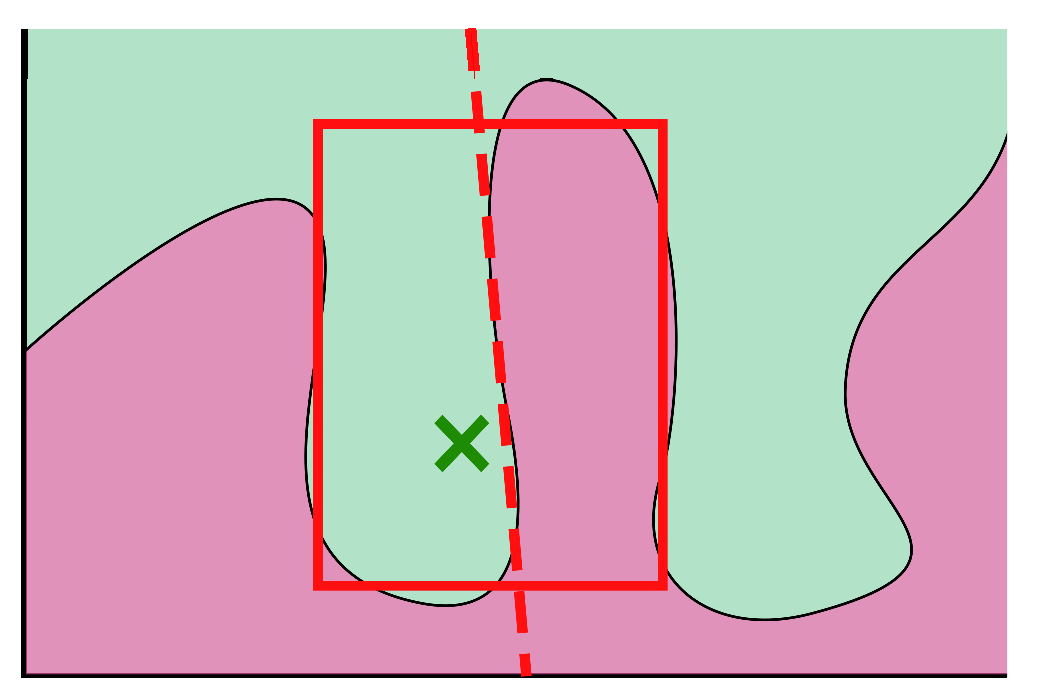
\includegraphics[width=0.39\textwidth]{visual-rlime3}
    \hspace{1em}
    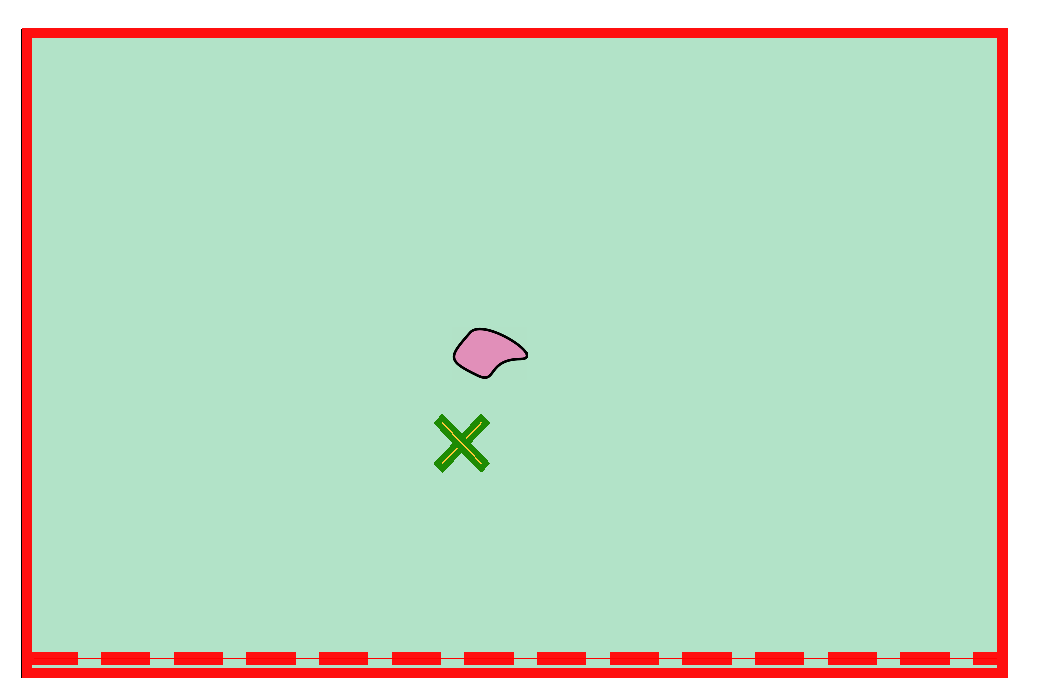
\includegraphics[width=0.4\textwidth]{visual-rlime-imbalanced}
  \end{figure}
  近似領域は入力空間全体になり,近似モデルは任意の入力を多数派クラスに分類
\end{frame}

\begin{frame}
  \frametitle{課題1の解決策}
  \begin{itemize}
    \item 損失関数を変更
          \begin{itemize}
            \item クラス比による重みづけ
            \item Focal Loss\footfullcite{lin2020focal}
          \end{itemize}
    \item ラベル分布の偏りを制約 \\
          \begin{itemize}
            \item 次の制約を追加
                  \begin{flalign*}
                    {\left(\mathbb{E}_{z\sim\mathcal{D}(z|A)}
                      [\mathbbm{1}_{f(z)=1}]-\frac{1}{2}\right)}^2<\mu
                  \end{flalign*}
          \end{itemize}
  \end{itemize}
\end{frame}

\begin{frame}
  \frametitle{課題2: 最適腕識別における報酬の分布の変化}
  KL-LUCBアルゴリズム\footfullcite{kaufmann2013information}による最適腕識別
  \begin{columns}[]
    \begin{column}{0.55\textwidth}
      \begin{itemize}
        \item 報酬の分布が不変であるという前提
        \item 近似モデルの更新によって,試行の度に報酬の分布が変化
      \end{itemize}
    \end{column}
    \begin{column}{0.5\textwidth}
      \begin{figure}
        \centering
        \includegraphics[width=0.9\textwidth]{src/bandit}
      \end{figure}
    \end{column}
  \end{columns}
\end{frame}

\begin{frame}
  \frametitle{課題2の検証}
  \begin{table}
    \small

    \begin{tabular}{cccc}
  \toprule
                     & Estimated acc. & True acc. & Deviation \\
  \midrule
  Average            & $.811$         & $.829$    & $.012$    \\
  Standard Deviation & $.018$         & $.023$    & $.017$    \\
  \bottomrule
\end{tabular}

    \caption{R-LIMEによる精度の推定値と真値の比較.}
  \end{table}

  信頼係数$1-\delta=0.95$を考慮すると,乖離の度合いは許容範囲内

  → 実用上は問題になりにくいが,選択アルゴリズムの改善が必要
\end{frame}

\end{document}
